\documentclass[10pt]{article}

\usepackage{csvsimple}
\usepackage{pgfplotstable}
\usepackage{longtable}
% recommended:
%\usepackage{booktabs}
%\usepackage{array}
%\usepackage{colortbl}
\usepackage{graphicx}

\usepackage[colorlinks,linkcolor={blue}]{hyperref}

\usepackage{nameref}
\usepackage{hyperref}

\title{Analysis of Project Time Series Data Performed in R}
\author{Stefan Kokov}

%----------------------------------------------------------------
% Path Variables
%----------------------------------------------------------------
\def \kokPlotsPath {../plots/}
\def \kokAcfPath {../acf/}
\def \kokPacfPath  {../pacf/}
\def \kokTestPath {../stationary_tests/}

\begin{document}
\maketitle



\section{Introduction and Methodology}
The analysis of the data set was performed using R tseries and urca packages.
ADF tests were performed using the ur.df function. Optimal number of lags were found using AIC information criteria. The PP tests were performed using the ur.pp function with $Z\tau$ statistic. The Stationary/Not stationary values in the tables below were derived by comparing the test statistic and the 5$\%$ confidence interval threshhold and they are not conclusive because rejection of the null hyphotesis is stronger than acceptance. Therefore the ADF and PP tests that result in Not Stationary conclusion show weaker results than the ones that result in a Stationary conclusion.

The structure of this report is as follows: \autoref{sec:ea} describes the variables of the EA data set, with discussion on the plot ACF, PACF and unit root test results for each variable. \autoref{sec:us} describes the variables of the US data set, with discussion on the plot ACF, PACF and unit root test results for each variable. \autoref{sec:conclusions} draws conclusions and suggests further working.



\pagebreak



\section{EA}
\label{sec:ea}


\subsection{CPI}
The CPI plot (\autoref{fig:ea_cpi}) shows large fluctuiations after around 2007 (probably caused by the Global Financial Crysis). This might be an indication that the time series is not stationary and the noise term accumulates. There doesn't seem to be much of a trend or seasonal component.

\begin{figure}[h!]
\centering
\includegraphics[width = 0.7\textwidth]{\kokPlotsPath ea_CPI}
\caption{plot EA CPI}
\label{fig:ea_cpi}
\end{figure}

Looking at the ACF (\autoref{fig:ea_cpi_acf}) of EA CPI, we see that it resembles thath of an Autoregressive model. The PACF doesn't show strong evidence of a moving average component, altough there are some minor fluctuations right after lag 0.

\begin{figure}[h!]
\centering
\includegraphics[width = 0.5\textwidth]{\kokAcfPath ea_CPI}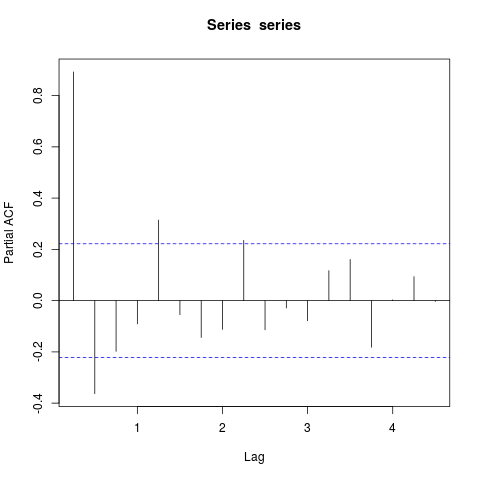
\includegraphics[width = 0.5\textwidth]{../pacf/ea_CPI}
\caption{ACF and PACF EA CPI}
\label{fig:ea_cpi_acf}
\end{figure}

\autoref{table:ea_cpi} Shows the results of the Stationarity tests ran on the EA CPI variable. The ADF test with drift and both KPSS tests suggest the series is stationary. However the ADF and KPSS with drift test results are very close to the 0.05 significance threshold. 

\begin{table}[h!]
\centering
\csvautotabular[respect all]{\kokTestPath ea_CPI.csv}
\caption{CPI EA Unit Root Tests}
\label{table:ea_cpi}
\end{table}



\subsection{GDP}

The plot of GDP (\autoref{fig:ea_gdp}) maybe suggests a downward trend. A fluctuation around 2008 is again ovserved. There is probably a drift as well.

\begin{figure}[h!]
\centering
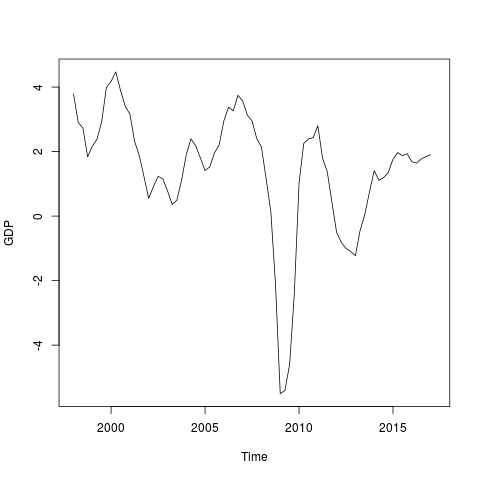
\includegraphics[width = 0.7\textwidth]{../plots/ea_GDP}
\caption{plot EA GDP}
\label{fig:ea_gdp}
\end{figure}

ACF and PCF (\autoref{fig:ea_gdp_acf}) again suggest an autoregressive model as expected.

\begin{figure}[h!]
\centering
\includegraphics[width = 0.5\textwidth]{\kokAcfPath ea_GDP}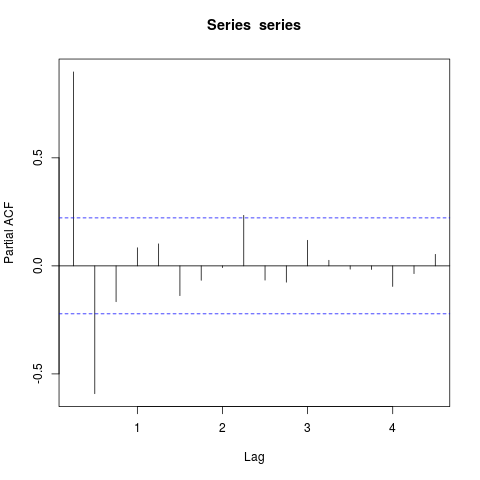
\includegraphics[width = 0.5\textwidth]{../pacf/ea_GDP}
\caption{ACF and PACF EA GDP}
\label{fig:ea_gdp_acf}
\end{figure}

The unit root test results (\autoref{table:ea_gdp}) suggest the series is stationary, maybe with a drift or/and trend. The KPSS results show it is not stationary which might be due to the changing varience around 2008.

\begin{table}[h!]
\centering
\csvautotabular[respect all]{\kokTestPath ea_GDP.csv}
\caption{GDP EA Unit Root Tests}
\label{table:ea_gdp}
\end{table}



\subsection{UR}

The EA unemployment rate curve (\autoref{fig:ea_ur}) looks very quite smooth, therefore the effect of the noise term in the model is insignificant. The mean is shifted so there is most probably a drift. There doesn't seem to be a particular trend.

\begin{figure}[h!]
\centering
\includegraphics[width = 0.7\textwidth]{\kokPlotsPath ea_UR}
\caption{plot EA UR}
\label{fig:ea_ur}
\end{figure}

UR ACF and PACF (\autoref{fig:ea_ur_acf}) show that there is a significant time dependance on previouse values of the variable. There might be an MA(1) element as well but this is not obvious.

\begin{figure}[h!]
\centering
\includegraphics[width = 0.5\textwidth]{\kokAcfPath ea_UR}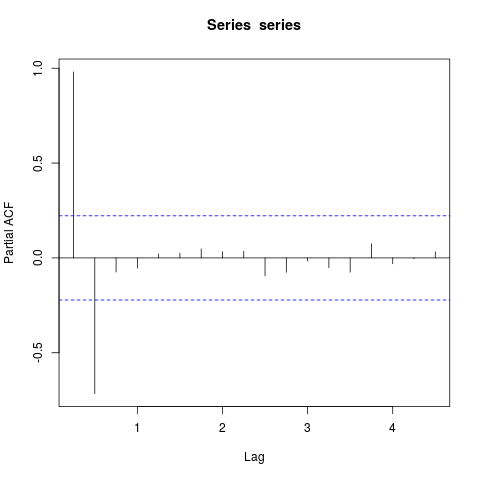
\includegraphics[width = 0.5\textwidth]{../pacf/ea_UR}
\caption{ACF and PACF EA UR}
\label{fig:ea_ur_acf}
\end{figure}

Only the KPSS tests suggest the variable is stationary (\autoref{table:ea_ur}), which isn't very strong evidence since rejection of the null hyphotesis is stronger than acceptance and none of the tests with non-stationary null (ADF and PP) tell us otherwise.

\begin{table}[h!]
\centering
\csvautotabular[respect all]{\kokTestPath ea_UR.csv}
\caption{UR EA Unit Root Tests}
\label{table:ea_ur}
\end{table}



\subsection{IR Policy Rate}

There deffinetly seems to be a downward trend in the EA IR Policy Rate variable (\autoref{fig:ea_irpolicyrate}).  It shows high but relativly constant variance. The mean is shifted.

\begin{figure}[h!]
\centering
\includegraphics[width = 0.7\textwidth]{"\kokPlotsPath ea_IR Policy Rate"}
\caption{plot EA IR Policy Rate}
\label{fig:ea_irpolicyrate}
\end{figure}

ACF and PACF (\autoref{fig:ea_irpolicyrate_acf}) exhibit the behaviour of an autoregressive model.

\begin{figure}[h!]
\centering
\includegraphics[width = 0.5\textwidth]{"\kokAcfPath ea_IR Policy Rate"}\includegraphics[width = 0.5\textwidth]{"../pacf/ea_IR Policy Rate"}
\caption{ACF and PACF EA IR Policy Rate}
\label{fig:ea_irpolicyrate_acf}
\end{figure}

The unit root tests (\autoref{fig:ea_irpolicyrate}) again show weak evidence of stationarity.

\begin{table}[h!]
\centering
\csvautotabular[respect all]{"\kokTestPath ea_IR Policy Rate.csv"}
\caption{IR Policy Rate EA Unit Root Tests}
\label{table:ea_irpolicyrate}
\end{table}



\subsection{LR10}

The EA LR10 variable has a distinct trend (\autoref{fig:ea_lr10-ir}). The mean is shifted and the decay might be considered exponential.

\begin{figure}[h!]
\centering
\includegraphics[width = 0.7\textwidth]{\kokPlotsPath ea_LR10}
\caption{plot EA LR10}
\label{fig:ea_lr10}
\end{figure}

ACF and PACF (\autoref{fig:ea_lr10_acf}) exhibit the typical behaviour of an autoregressive model.

\begin{figure}[h!]
\centering
\includegraphics[width = 0.5\textwidth]{\kokAcfPath ea_LR10}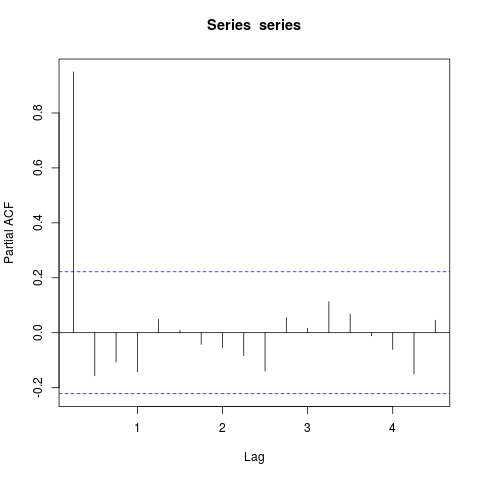
\includegraphics[width = 0.5\textwidth]{../pacf/ea_LR10}
\caption{ACF and PACF EA LR10}
\label{fig:ea_lr10_acf}
\end{figure}

Again only the KPSS tests show the variable might be stationary (\autoref{table:ea_lr10}).

\begin{table}[h!]
\centering
\csvautotabular[respect all]{"\kokTestPath ea_LR10.csv"}
\caption{LR10 EA Unit Root Tests}
\label{table:ea_lr10}
\end{table}



\subsection{LR10-IR}

The LR10-IR (\autoref{fig:ea_lr10-ir}) derived variable seems to have some periodic behaviour. A particular trend doesn't seem to be present. The mean is shifted.

\begin{figure}[h!]
\centering
\includegraphics[width = 0.7\textwidth]{\kokPlotsPath ea_LR10-IR}
\caption{plot EA LR10-IR}
\label{fig:ea_lr10-ir}
\end{figure}

The ACF (\autoref{fig:ea_lr10-ir_acf}) shows a strong autocorelation even for lags after the initial decay. 

\begin{figure}[h!]
\centering
\includegraphics[width = 0.5\textwidth]{\kokAcfPath ea_LR10-IR}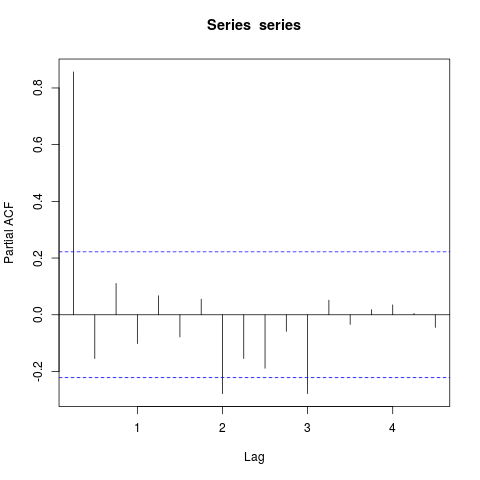
\includegraphics[width = 0.5\textwidth]{../pacf/ea_LR10-IR}
\caption{ACF and PACF EA LR10-IR}
\label{fig:ea_lr10-ir_acf}
\end{figure}

Again weak evidence of stationarity from the tests (\autoref{table:ea_lr10-ir}).

\begin{table}[h!]
\centering
\csvautotabular[respect all]{"\kokTestPath ea_LR10-IR.csv"}
\caption{LR10-IR EA Unit Root Tests}
\label{table:ea_lr10-ir}
\end{table}



\subsection{Exchange Rate EUR to USD}
\label{subsec:exrate}

The exchange rate between euro and dollar (\autoref{fig:ea_exrateEURtoUSD}) has a non zero mean as expected. A trend is not present. There is some periodic behaviour but doesn't seem to be seasonal.

\begin{figure}[h!]
\centering
\includegraphics[width = 0.7\textwidth]{"\kokPlotsPath ea_Exrate Euro for 1 USD"}
\caption{plot EA Exchange Rate EUR to USD}
\label{fig:ea_exrateEURtoUSD}
\end{figure}

ACF and PACF (\autoref{fig:ea_exrateEURtoUSD_acf}) are typical for an autoregressive variable.

\begin{figure}[h!]
\centering
\includegraphics[width = 0.5\textwidth]{"\kokAcfPath ea_Exrate Euro for 1 USD"}\includegraphics[width = 0.5\textwidth]{"../pacf/ea_Exrate Euro for 1 USD"}
\caption{ACF and PACF EA Exchange Rate EUR to USD}
\label{fig:ea_exrateEURtoUSD_acf}
\end{figure}

Weak evidence of stationarity from unit root tests (\autoref{table:ea_exrate})

\begin{table}[h!]
\centering
\csvautotabular[respect all]{"\kokTestPath ea_Exrate Euro for 1 USD.csv"}
\caption{Exchange Rate EA Unit Root Tests}
\label{table:ea_exrate}
\end{table}



\pagebreak



\section{US}
\label{sec:us}

\subsection{CPI}

The US CPI plot (\autoref{fig:us_cpi}) shows evidence of a drift term but no trend. There is again a spike around 2009 but apart from that variance seems to be constant.

\begin{figure}[h!]
\centering
\includegraphics[width = 0.7\textwidth]{\kokPlotsPath us_CPI}
\caption{plot US CPI}
\label{fig:us_cpi}
\end{figure}

ACF and PACF plots (\autoref{fig:us_cpi_acf}) show behaviour of autoregressive model with some fluctuiations in the PACF.

\begin{figure}[h!]
\centering
\includegraphics[width = 0.5\textwidth]{\kokAcfPath us_CPI}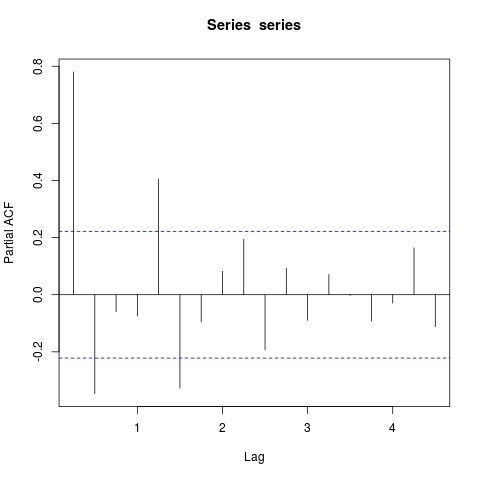
\includegraphics[width = 0.5\textwidth]{../pacf/us_CPI}
\caption{ACF and PACF US CPI}
\label{fig:us_cpi_acf}
\end{figure}

Unit root tests (\autoref{table:us_cpi}) good show evidence of stationarity from both PP and ADF tests.

\begin{table}[h!]
\centering
\csvautotabular[respect all]{\kokTestPath us_CPI.csv}
\caption{CPI US Unit Root Tests}
\label{table:us_cpi}
\end{table}


\subsection{GDP}

The plot of US GDP (\autoref{fig:us_gdp}) shows a mean close to zero. A clear trend cannot be seen. Fluctuation around the Global financial crysis is present again.

\begin{figure}[h!]
\centering
\includegraphics[width = 0.7\textwidth]{\kokPlotsPath us_GDP}
\caption{plot US GDP}
\label{fig:us_gdp}
\end{figure}

An autoregressive model with a dependance on relativly few lags is suggested by the ACF and PACF (\autoref{fig:us_gdp_acf})

\begin{figure}[h!]
\centering
\includegraphics[width = 0.5\textwidth]{\kokAcfPath us_GDP}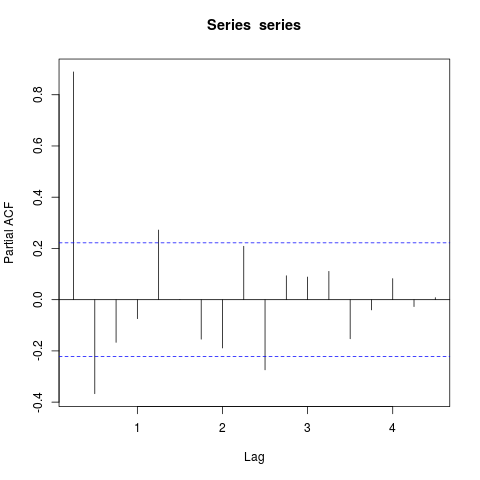
\includegraphics[width = 0.5\textwidth]{../pacf/us_GDP}
\caption{ACF and PACF US GDP}
\label{fig:us_gdp_acf}
\end{figure}

Strong evidence of stationarity by both ADF and KPSS tests (\autoref{table:us_gdp}).

\begin{table}[h!]
\centering
\csvautotabular[respect all]{\kokTestPath us_GDP.csv}
\caption{ US Unit Root Tests}
\label{table:us_gdp}
\end{table}

\subsection{UR}

Unemployment rate cureve (\autoref{fig:us_ur}) is again very smooth as the EA one. The plot suggests an exponential frowth. The mean is shifted so there is probably drift. 

\begin{figure}[h!]
\centering
\includegraphics[width = 0.7\textwidth]{\kokPlotsPath us_UR}
\caption{plot US UR}
\label{fig:us_ur}
\end{figure}

Strong autocorrelation in ACF (\autoref{fig:us_ur_acf}).

\begin{figure}[h!]
\centering
\includegraphics[width = 0.5\textwidth]{\kokAcfPath us_UR}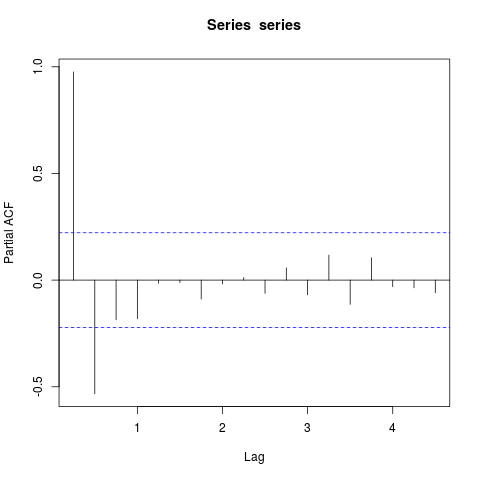
\includegraphics[width = 0.5\textwidth]{../pacf/us_UR}
\caption{ACF and PACF US UR}
\label{fig:us_ur_acf}
\end{figure}

Stationarity test results (\autoref{table:us_ur}) not very convincing. Only KPSS tests suggest stationarity. 

\begin{table}[h!]
\centering
\csvautotabular[respect all]{\kokTestPath us_UR.csv}
\caption{UR US Unit Root Tests}
\label{table:us_ur}
\end{table}


\subsection{IR FEDFUNDS}

US IR variable (\autoref{fig:us_ir10fedfunds}) shows high variance followed by a period of low variance. Drift is present. There is some evidence of a trend.

\begin{figure}[h!]
\centering
\includegraphics[width = 0.7\textwidth]{"\kokPlotsPath us_IR FEDFUNDS"}
\caption{plot US IR10 fedfunds}
\label{fig:us_ir10fedfunds}
\end{figure}

Again typical autoregressive model ACF and PACF (\autoref{fig:us_ir10fedfunds-ir_acf})

\begin{figure}[h!]
\centering
\includegraphics[width = 0.5\textwidth]{"\kokAcfPath us_IR FEDFUNDS"}\includegraphics[width = 0.5\textwidth]{"../pacf/us_IR FEDFUNDS"}
\caption{ACF and PACF US IR10 fedfunds}
\label{fig:us_ir10fedfunds-ir_acf}
\end{figure}

Evidence of stationarity from both ADF and KPSS tests (\autoref{table:us_ir}). A

\begin{table}[h!]
\centering
\csvautotabular[respect all]{"\kokTestPath us_IR FEDFUNDS.csv"}
\caption{IR Fedfunds US Unit Root Tests}
\label{table:us_ir}
\end{table}

\subsection{IR10 premium}

IR10 premium variable plot (\autoref{fig:us_ir10prem}) show decaying variance. There is no apperant trend.

\begin{figure}[h!]
\centering
\includegraphics[width = 0.7\textwidth]{"\kokPlotsPath us_IR10 premium"}
\caption{plot US IR10 premium}
\label{fig:us_ir10prem}
\end{figure}

Autocorrelations of lags much after initial decline in ACF (\autoref{fig:us_ir10prem-ir_acf}).

\begin{figure}[h!]
\centering
\includegraphics[width = 0.5\textwidth]{"\kokAcfPath us_IR10 premium"}\includegraphics[width = 0.5\textwidth]{"../pacf/us_IR10 premium"}
\caption{ACF and PACF US IR10 premium}
\label{fig:us_ir10prem-ir_acf}
\end{figure}

No evidence of stationarity from any of the tests (\autoref{table:us_ir10})

\begin{table}[h!]
\centering
\csvautotabular[respect all]{"\kokTestPath us_IR10 premium.csv"}
\caption{IR 10 premium US Unit Root Tests}
\label{table:us_ir10}
\end{table}

\subsection{LR10 - IR}

The plot of the LR10 - IR (\autoref{fig:us_lr10-ir}) suggests a very clear downward trend. Variance is relativly constant. There might be some seasonal behaviour but it is not obvious.

\begin{figure}[h!]
\centering
\includegraphics[width = 0.7\textwidth]{"\kokPlotsPath us_LR10 - IR"}
\caption{plot US LR10 - IR}
\label{fig:us_lr10-ir}
\end{figure}

Strong autocorrelation in ACF on many lags (\autoref{fig:us_lr10-ir_acf}).

\begin{figure}[h!]
\centering
\includegraphics[width = 0.5\textwidth]{"\kokAcfPath us_LR10 - IR"}\includegraphics[width = 0.5\textwidth]{"../pacf/us_LR10 - IR"}
\caption{ACF and PACF US LR10 - IR}
\label{fig:us_lr10-ir_acf}
\end{figure}

Weak evidence of stationarity from only KPSS unit root test (\autoref{table:us_lr10-ir})

\begin{table}[h!]
\centering
\csvautotabular[respect all]{"\kokTestPath us_LR10 - IR.csv"}
\caption{LR10-IR US Unit Root Tests}
\label{table:us_lr10-ir}
\end{table}


\subsection{Exchange Rate USD to EUR}

Exchange rate USD to EUR is the naturally the opposite of EUR to USD (\autoref{subsec:exrate}) , therefore the properties are equivalent (\autoref{fig:us_exrateUSDtoEUR}, \autoref{fig:us_exrateUSDtoEUR_acf}, \autoref{table:us_exrate}).

\begin{figure}[h!]
\centering
\includegraphics[width = 0.7\textwidth]{"\kokPlotsPath us_Exrate USD to 1 Euro"}
\caption{plot US Exchange Rate USD to EUR}
\label{fig:us_exrateUSDtoEUR}
\end{figure}

\begin{figure}[h!]
\centering
\includegraphics[width = 0.5\textwidth]{"\kokAcfPath us_Exrate USD to 1 Euro"}\includegraphics[width = 0.5\textwidth]{"../pacf/us_Exrate USD to 1 Euro"}
\caption{ACF and PACF US Exchange Rate USD to EUR}
\label{fig:us_exrateUSDtoEUR_acf}
\end{figure}

\begin{table}[h!]
\centering
\csvautotabular[respect all]{"\kokTestPath us_Exrate USD to 1 Euro.csv"}
\caption{Exchange Rate US Unit Root Tests}
\label{table:us_exrate}
\end{table}

\pagebreak

\section{Conclusions}
\label{sec:conclusions}
The majority of variables don't exhibit strong evidence of stationarity. Further tests need to be performed with different preprocessing techniques. The effect of differencing and/or log transformations needs to be tested. There are fluctuations in the data around the global financial crisis which cause high variance. These fluctuations along with the small sample size of the data cause it to exhibit non stationary behaviour even for variable that have long been theorised to be stationary by economist - CPI. Furthermore the performance of ADF and PP tests is sensitive to the sample size and do not perform very well on small data samples such as the one used.

\end{document}